\documentclass[man,floatsintext]{apa6}
\usepackage{lmodern}
\usepackage{amssymb,amsmath}
\usepackage{ifxetex,ifluatex}
\usepackage{fixltx2e} % provides \textsubscript
\ifnum 0\ifxetex 1\fi\ifluatex 1\fi=0 % if pdftex
  \usepackage[T1]{fontenc}
  \usepackage[utf8]{inputenc}
\else % if luatex or xelatex
  \ifxetex
    \usepackage{mathspec}
  \else
    \usepackage{fontspec}
  \fi
  \defaultfontfeatures{Ligatures=TeX,Scale=MatchLowercase}
\fi
% use upquote if available, for straight quotes in verbatim environments
\IfFileExists{upquote.sty}{\usepackage{upquote}}{}
% use microtype if available
\IfFileExists{microtype.sty}{%
\usepackage{microtype}
\UseMicrotypeSet[protrusion]{basicmath} % disable protrusion for tt fonts
}{}
\usepackage{hyperref}
\hypersetup{unicode=true,
            pdftitle={Drought frequency predicts life history strategies in Heliophila},
            pdfauthor={J. Grey Monroe, Brian Gill, Kathryn G. Turner, \& John K. McKay},
            pdfkeywords={drought adaptation, life history evolution, remote sensing,
phylogeography, herbaria records},
            pdfborder={0 0 0},
            breaklinks=true}
\urlstyle{same}  % don't use monospace font for urls
\usepackage{graphicx,grffile}
\makeatletter
\def\maxwidth{\ifdim\Gin@nat@width>\linewidth\linewidth\else\Gin@nat@width\fi}
\def\maxheight{\ifdim\Gin@nat@height>\textheight\textheight\else\Gin@nat@height\fi}
\makeatother
% Scale images if necessary, so that they will not overflow the page
% margins by default, and it is still possible to overwrite the defaults
% using explicit options in \includegraphics[width, height, ...]{}
\setkeys{Gin}{width=\maxwidth,height=\maxheight,keepaspectratio}
\IfFileExists{parskip.sty}{%
\usepackage{parskip}
}{% else
\setlength{\parindent}{0pt}
\setlength{\parskip}{6pt plus 2pt minus 1pt}
}
\setlength{\emergencystretch}{3em}  % prevent overfull lines
\providecommand{\tightlist}{%
  \setlength{\itemsep}{0pt}\setlength{\parskip}{0pt}}
\setcounter{secnumdepth}{0}
% Redefines (sub)paragraphs to behave more like sections
\ifx\paragraph\undefined\else
\let\oldparagraph\paragraph
\renewcommand{\paragraph}[1]{\oldparagraph{#1}\mbox{}}
\fi
\ifx\subparagraph\undefined\else
\let\oldsubparagraph\subparagraph
\renewcommand{\subparagraph}[1]{\oldsubparagraph{#1}\mbox{}}
\fi

%%% Use protect on footnotes to avoid problems with footnotes in titles
\let\rmarkdownfootnote\footnote%
\def\footnote{\protect\rmarkdownfootnote}


  \title{Drought frequency predicts life history strategies in \emph{Heliophila}}
    \author{J. Grey Monroe\textsuperscript{1,2}, Brian Gill\textsuperscript{3},
Kathryn G. Turner\textsuperscript{4}, \& John K.
McKay\textsuperscript{2}}
    \date{}
  
\shorttitle{Drought and life history}
\affiliation{
\vspace{0.5cm}
\textsuperscript{1} Graduate Degree Program in Ecology, Colorado State University, Fort Collins, CO 80521, USA\\\textsuperscript{2} College of Agriculture, Colorado State University, Fort Collins, CO 80521, USA\\\textsuperscript{3} Institute for Environment and Society, Brown University, Providence, RI 02912, USA\\\textsuperscript{4} Biology Department, Pennsylvania State University, State College, PA 16802, USA}
\keywords{drought adaptation, life history evolution, remote sensing, phylogeography, herbaria records}
\usepackage{csquotes}
\usepackage{upgreek}
\captionsetup{font=singlespacing,justification=justified}

\usepackage{longtable}
\usepackage{lscape}
\usepackage{multirow}
\usepackage{tabularx}
\usepackage[flushleft]{threeparttable}
\usepackage{threeparttablex}

\newenvironment{lltable}{\begin{landscape}\begin{center}\begin{ThreePartTable}}{\end{ThreePartTable}\end{center}\end{landscape}}

\makeatletter
\newcommand\LastLTentrywidth{1em}
\newlength\longtablewidth
\setlength{\longtablewidth}{1in}
\newcommand{\getlongtablewidth}{\begingroup \ifcsname LT@\roman{LT@tables}\endcsname \global\longtablewidth=0pt \renewcommand{\LT@entry}[2]{\global\advance\longtablewidth by ##2\relax\gdef\LastLTentrywidth{##2}}\@nameuse{LT@\roman{LT@tables}} \fi \endgroup}


\usepackage{lineno}

\linenumbers
\newcommand{\beginsupplement}{\setcounter{table}{0}  \renewcommand{\thetable}{S\arabic{table}} \setcounter{figure}{0} \renewcommand{\thefigure}{S\arabic{figure}}}

\authornote{

Correspondence concerning this article should be addressed to J. Grey
Monroe, 307 University Ave, Fort Collins, CO 80521. E-mail:
\href{mailto:monroejg@colostate.edu}{\nolinkurl{monroejg@colostate.edu}}}

\abstract{
Explaining variation in life history strategies is a long-standing goal
of evolutionary biology. For plants, annual and perennial life histories
are thought to reflect adaptation to environments that differ in the
frequency of environmental stress such as drought. Here we test this
hypothesis in \textit{Heliophila} (Brassicaceae), a diverse genus of
flowering plants native to Africa, by integrating 34 years of
satellite-based drought measurements with 2192 herbaria occurrence
records. Consistent with predictions from classic life history theory,
we find that perennial \textit{Heliophila} species occur in environments
where droughts are significantly less frequent compared to annuals.
These associations are predictive while controlling for phylogeny,
lending support to the hypothesis that drought related natural selection
has influenced the distributions of these strategies. Additionally, the
difference in drought frequency between annual and perennial species
distributions is greatest during the summer and fall, which also appears
to be when annuals are in the seed phase of their life cycle based on
collection dates of annual species. Together, these finding provide
empirical support for classic hypotheses about the drivers of life
history strategy in plants - that perennials out compete annuals in
environments with less frequent drought and that annuals are adapted to
environments with more frequent drought by escaping drought prone
seasons as seeds. 
}

\usepackage{amsthm}
\newtheorem{theorem}{Theorem}[section]
\newtheorem{lemma}{Lemma}[section]
\theoremstyle{definition}
\newtheorem{definition}{Definition}[section]
\newtheorem{corollary}{Corollary}[section]
\newtheorem{proposition}{Proposition}[section]
\theoremstyle{definition}
\newtheorem{example}{Example}[section]
\theoremstyle{definition}
\newtheorem{exercise}{Exercise}[section]
\theoremstyle{remark}
\newtheorem*{remark}{Remark}
\newtheorem*{solution}{Solution}
\begin{document}
\maketitle

\hypertarget{introduction}{%
\section{Introduction}\label{introduction}}

Understanding the causes and consequences of life history variation is a
longstanding goal of ecology and evolutionary biology (Cole, 1954). In
plants, life histories are especially diverse, with herbaceous species
that complete their life cycle in a number of weeks to trees that live
for thousands of years (Brown, 1996). Along this continuum an important
division exists, distinguishing annuals which complete their seed to
seed life cycle within a single calendar year from perennials which can
persist over multiple years. Annual plants flower once, set seed,
senesce, and then die, spending at least some portion of the year as a
seed, where they are relatively protected from environmental stress. In
contrast, perennial plants can continue vegetative growth after
reproduction and must survive conditions experienced during all seasons.
These represent fundamentally different life history strategies, but the
ecological factors that explain their evolution and distributions remain
empirically uresolved (Friedman and Rubin, 2015).\\
Classical theory predict shorter life spans in environments where adult
mortality is high (Charnov and Schaffer, 1973; Franco and Silvertown,
1996; Stearns, 1992). In plants, this has been extended to the
hypothesis that annuality is adaptive when it allows plants to escape
drought (Schaffer and Gadgil, 1975). Lack of water is perhaps the
greatest threat to survival during vegetative or reproductive growth and
annuals can remain dormant (and protected as a seed) during drought.
Thus, environments with greater seasonal drought frequency may select
for annual life histories that complete reproduction prior to drought
prone seasons. Conversely, environments with less frequent drought may
select for perennial species, which may benefit from multiple bouts of
reproduction and competitive advantage by preventing recruitment of
annual species (Corbin and D'Antonio, 2004). These predictions have been
supported by the observation of annuals in arid environments in
\emph{Oryza perennis} (Morishima et al., 1984) and \emph{Oenothera}
(Evans et al., 2005). Additionally, annual and perennial species of
\emph{Nemesia} were qualitatively associated with winter rather and
summer rainfall environments respectively (Datson et al., 2008) and
annual species of \emph{Scorzoneroides} were associated with
environments classified as unpredictable (Cruz-Mazo et al., 2009).
However, whether the history frequency of drought events indeed predicts
the distributions annual or perennial life history strategies has yet to
be tested.\\
Here we combine a long-term global dataset of satellite detected drought
events with metadata from natural history collections to test these
classic hypotheses within the African endemic mustard genus,
\emph{Heliophila} L. (Brassicaceae). If annuality is an adaptive
strategy allowing plants to escape drought prone seasons, then drought
frequency should predict the distribution of life history strategies
across landscapes, and annual species should be more commonly associated
with drought prone regions than perennial species. Furthermore, if
annual species have adapted to escape drought prone seasons,
observations of growing annual species (i.e.~occurring in forms other
than seed) should be rare during drought prone seasons. Phylogenetic
relatedness can influence tests of associations between species' traits
and their environments (Barrett et al., 1996; Felsenstein, 1985), and
therefore we assessed the relationship between life history distribution
and drought frequency in a phylogenetic context.

\hypertarget{materials-and-methods}{%
\section{Materials and Methods}\label{materials-and-methods}}

\hypertarget{data}{%
\subsection{Data}\label{data}}

\hypertarget{availability}{%
\subsubsection{Availability}\label{availability}}

All analyses were performed using R. All data and the source code to
produce this manuscript are available at
\url{https://github.com/greymonroe/heliophila}. Software used is listed
in the supplement.

\hypertarget{satellite-detected-drought-data}{%
\subsubsection{Satellite-detected drought
data}\label{satellite-detected-drought-data}}

Remotely sensed data is a powerful tool for characterizing seasonal
patterns in drought because it is less limited in spatial and temporal
scope and resolution than weather stations or field observations
(AghaKouchak et al., 2015). To quantify the frequency of drought during
different seasons across landscapes, we used the remotely sensed
Vegetative Health Index (VHI), which measures landscape scale reductions
in plant cover and temperature conditions characteristic of drought
(Kogan, 2001). Generated from data collected by NOAA AVHRR satellites
since 1981, the VHI combines Normalized Difference Vegetation Index
(NDVI) derived measures of vegetative stress (Vegetative Condition Index
- VCI) with temperature stress indicated by anomalies in thermal spectra
(Temperature Condition Index - TCI). The VHI of year \(y\) during week
\(w\) of \([1,52]\) at pixel \(i\) is derived from the following
equations, where \(n\) is the number of years observed.

\[VCI_{y,w,i} = 100\frac{NDVI_{y,w,i} - NDVI_{min}}{NDVI_{max} - NDVI_{min}}\]

\[TCI_{y,w,i} = 100\frac{T_{y,w,i} - T_{min}}{T_{max} - T_{min}}\]

\[VHI_{y,w,i} = 0.5(VCI_{y,w,i}) + 0.5(TCI_{y,w,i})\] where
\(NDVI_{min} = min(NDVI_{1981,w,i}...NDVI_{1981+n,w,i})\) and
\(NDVI_{max} = max(NDVI_{1981,w,i}...NDVI_{1981+n,w,i})\) and
\(T_{min} = min(T_{1981,w,i}...T_{1981+n,w,i})\) and
\(T_{max} = max(T_{1981,w,i}...T_{1981+n,w,i})\)

Thus, VHI measurements are standardized according to conditions
historically observed at each locations. These measurements have been
validated and generally used for evaluating drought risk and predicting
crop yields in agriculture (e.g., Rojas et al., 2011; Kogan et al.,
2016). But they also present a new tool to study seasonal patterns in
the frequency of drought across environments and to test hypotheses
about the effect of drought on ecological and evolutionary processes
(Kerr and Ostrovsky, 2003). As such, the VHI has been applied recently
to study drought related ecology of natural species and proven useful
for predicting intraspecific variation in drought tolerance traits and
genes (Dittberner et al., 2018; Mojica et al., 2016; J. Monroe, Powell,
et al., 2018). Here, we accessed VHI data at \(16km^2\) resolution from
1981 to 2015
(\url{https://www.star.nesdis.noaa.gov/smcd/emb/vci/VH/vh_ftp.php}) to
characterize the seasonal drought frequencies experienced by annual and
perennial \emph{Heliophila} species.

\hypertarget{life-history-data-for-heliophila}{%
\subsubsection{\texorpdfstring{Life history data for
\emph{Heliophila}}{Life history data for Heliophila}}\label{life-history-data-for-heliophila}}

\emph{Heliophila} is a genus of flowering plants endemic to the southern
portion of Africa including the Cape Floristic and Succulent Karoo
Regions. These are among the most botanically diverse environments on
Earth and the \emph{Heliophila} species occurring there are considered
to make up the most diverse genus of the family Brassicaceae (Mandáková
et al., 2012; Mummenhoff et al., 2005). This genus includes both
perennial and annual species and this change in life history strategy
has likely arisen multiple independent times (Appel and Al-Shehbaz,
1997; Mummenhoff et al., 2005). Furthermore, the fine scale climatic
heterogeneity of Southern Africa is ideal for studying the distribution
of traits in relation to environmental parameters (Sayre et al., 2013).
We used life histories reported by Mummenhoff et al. (2005), grouping
species with annual or perennial life histories. Perenniality was
defined based any form of perennial life history (e.g., herbs, shrubs,
mixed, etc). Because the nature of species reported with mixed traits
were unknown (i.e.~plasticity vs.~genetic variation), we classified
these species here as perennial since they can maintain vegetative
growth after reproduction at least to some capacity.

\hypertarget{heliophila-occurrence-records}{%
\subsubsection{\texorpdfstring{\emph{Heliophila} occurrence
records}{Heliophila occurrence records}}\label{heliophila-occurrence-records}}

Botanists have collected and maintained over 350 million botanical
specimens worldwide over the past 300 years. Herbarium specimens and
their associated metadata have been used since the 1960s to study
species' geographical distributions (reviewed by Willis et al. (2017)
and Lang et al. (2018)). And as they become digitized (Soltis, 2017),
these collections have been used to study relationships between trait
distributions, geography, and climate (Davis et al., 2015; Stropp et
al., 2016; Václavı'k et al., 2017; Wolf et al., 2016). To characterize
the distributions of annual and perennial \emph{Heliophila} species, all
records for the genus \emph{Heliophila} were downloaded from the Global
Biodiversity Information Facility (gbif.org) on July 21, 2018 (GBIF,
2018).

\hypertarget{sequence-data-for-phylogeny}{%
\subsubsection{Sequence data for
phylogeny}\label{sequence-data-for-phylogeny}}

An alignment of ITS I and II sequences for \emph{Heliophila} species was
obtained from the authors of Mandáková et al. (2012). Individual ITS I
and II sequences for \emph{Aethionema grandiflorum, Alliaria petiolata,
Cardamine matthioli, Chamira circaeoides}, and \emph{Rorippa amphibia}
were downloaded from Genbank.

\hypertarget{analyses}{%
\subsection{Analyses}\label{analyses}}

\hypertarget{drought-frequency-calculations}{%
\subsubsection{Drought frequency
calculations}\label{drought-frequency-calculations}}

To characterize drought regimens across the distributions of annual and
perennial species of \emph{Heliophila}, we calculated drought during
different seasons at the location of observations for \emph{Heliophila}
records using the VHI. Specifically, we created global maps of the
frequencies of observing drought conditions (VHI\textless{}40, NOAA)
during the winter (quarter surrounding winter solstice), spring (quarter
surrounding spring equinox), summer (quarter surrounding summer
solstice) and fall (quarter surrounding fall equinox) from 1981 to 2015.
From these maps, the drought frequency during the winter, spring,
summer, and fall were extracted for the locations of all GBIF records.

\hypertarget{filtering-of-occurrence-records}{%
\subsubsection{Filtering of occurrence
records}\label{filtering-of-occurrence-records}}

To avoid instances with spurious location data, we filtered raw GBIF by
restricting our analyses to include only:

\begin{itemize}
\tightlist
\item
  records for species with reported life history\\
\item
  records with geospatial data\\
\item
  records without known geospatial coordinate issues (i.e., coordinates
  reported are those of herbarium)\\
\item
  records from collection sites classified as land pixels\\
\item
  records from Africa (to exclude locations of cultivation)
\item
  records without duplicates (i.e., identical species, location,
  collection date)
\end{itemize}

\hypertarget{phylogeny-construction}{%
\subsubsection{Phylogeny construction}\label{phylogeny-construction}}

Out group ( \emph{Aethionema grandiflorum, Alliaria petiolata, Cardamine
matthioli, Chamira circaeoides}, and \emph{Rorippa amphibia}) and
ingroup \emph{Heliophila} ITS I and II sequences were aaligned using
MAFFT (Katoh et al., 2002) with strategy G-INS-I, offset value 0.1, and
all other options set as default. The \(GTR + L\) model of nucleotide
substitution was determined to best fit the data based on AIC using
jModelTest2 (Darriba et al., 2012; Guindon and Gascuel, 2003). A maximum
clade credibility tree with branch lengths as relative time was
estimated by summarizing data from six runs of 100,000,000 generations
of Bayesian Markov chain Monte Carlo conducted in BEAST 2 (Bouckaert et
al., 2014). Model selection and phylogenetic analyses were conducted
through the CIPRES Science Gateway (Miller et al., 2010).

\hypertarget{comparison-of-drought-frequency-between-annual-and-perennial-species}{%
\subsubsection{Comparison of drought frequency between annual and
perennial
species}\label{comparison-of-drought-frequency-between-annual-and-perennial-species}}

To evaluate the hypothesis that annual and perennial life history
strategies reflect adaptations to alternative drought regimes, we tested
the corresponding prediction that the observed distributions of annual
and perennial \emph{Heliophila} species would be significantly
associated with historic drought frequency. First, we compared the
frequency of drought during the winter, spring, summer, and fall between
raw occurrence records of annual and perennial species by t-tests. To
account for variation in the number of occurrence records per species,
we next calculated the mean drought frequency during the winter, spring,
summer and fall for each species. Because shared evolutionary history of
closely related species can lead to spurious associations between traits
and environments (Felsenstein, 1985), we tested for a relationship
between life history strategy and drought frequency while controlling
for phylogeny using phylogenetic logistic regression (Ives and Garland,
2010).

\hypertarget{collection-dates}{%
\subsubsection{Collection dates}\label{collection-dates}}

To test the hypothesis that annual species have adapted to escape
drought prone seasons as seeds, collection dates for herbarium specimens
were compared between annual and perennial species. Comparisons of
distributions were made by Two-sample Kolmogorov-Smirnov test, t-test,
and Barlett variance test.

\hypertarget{results}{%
\section{Results}\label{results}}











\begin{figure}[!h]
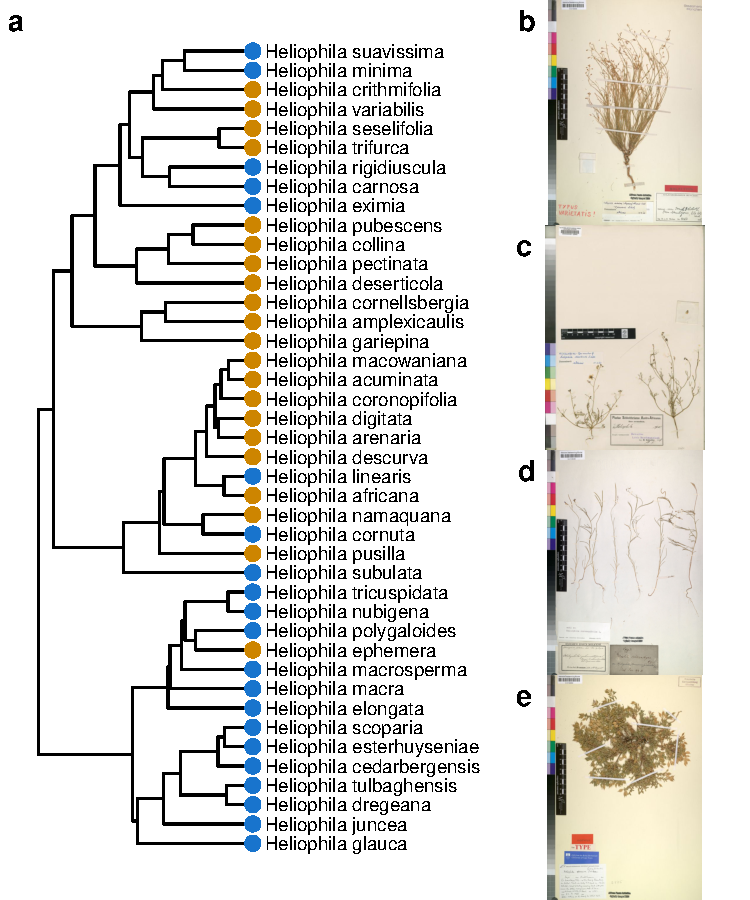
\includegraphics[width=\textwidth]{../figures/phylogeny} \caption{Species and examples of herbaria specimens of
\emph{Heliophila} (a) Phylogeny and life history strategies of species
studied. Orange circles at branch tips mark annual species and blue
circles mark perennial species. Example herbaria specimens accessed via
GBIF of (a) \emph{H. minima}, (b) \emph{H. deserticola}, (c) \emph{H.
coronopifolia} and (d) \emph{H. ephemera}. Images (a,c,d) courtesy of
The Bavarian Natural History Collections (CC BY-SA 4.0) and (b) The
London Natural History Museum (CC BY 4.0). Links to images are found in
the supplement.}\label{fig:phylogeny}
\end{figure}







\begin{figure}[!h]
\includegraphics[width=\textwidth]{../figures/maps_boxplots} \caption{Locations of occurrence records of (a) annual and (b)
perennial \emph{Heliophila.} Drought frequency during the (c) winter,
(d) spring, (e) summer and (f) fall measured using the VHI. (g) Drought
frequencies during each season at the observation locations of annual
and perennial \emph{Heliophila} (t tests, ** = p \textless{} 0.01).}\label{fig:mapsboxplots}
\end{figure}

Out of 8670 \emph{Heliophila} GBIF records, 6634 were for species with
reported life history (Mummenhoff et al., 2005), 2856 had geospatial
data, 2833 did not have geospatial issues, 2684 were located on pixels
classified as land having drought measurements, 2543 were located in
Africa, 2192 were not duplicated. Thus, after all filtering steps, 2192
records for 42 species (Figure \ref{fig:phylogeny}, Table
\ref{tab:speciesmeanstable}) passed for further analyses. The number of
samples varied between species, with a mean of 52.19 samples per
species. Heliophila rigidiuscula had the most records, 201, and
Heliophila cornellsbergia the fewest, 2 (Table
\ref{tab:speciesmeanstable}).

There were clear visual differences between the distributions of the 960
annual and the 1232 perennial \emph{Heliophila} observation records (see
Figure \ref{fig:speciesmaps} for maps of individual species). While
annual species were generally found in the western regions of South
Africa and Namibia, primarily in the Cape Floristic Region and Succulent
Karoo (Figure \ref{fig:mapsboxplots}a), the occurrence of perennials
extended to the east coast of South Africa (Figure
\ref{fig:mapsboxplots}b).

The frequency of drought varied considerably across the ranges of
\emph{Heliophila} species (Figure \ref{fig:mapsboxplots}c-f). This
heterogeneity is expected, given that this is one of the most
climatically diverse regions of the Earth (Sayre et al., 2013). It is
worth noting the east to west cline in drought frequency observed during
the summer, which distinguishes the high drought frequency of the
Kalahari Sands and Namid Desert phytogeographic regions from the low
drought frequency of the Drakensberg Mountains and Coastal Zambesian
phytogeographic regions. In the Cape phytogeographic region there was
finer scale heterogeneity in drought frequency during the summer.

Theory predicts that annuality should be adaptive in places where
stresses such as drought are more common. Conversely, perenniality
should be adaptive in places where such stresses are less frequent. We
found that the frequency of drought was significantly higher at the
locations of occurrence records for annual species. In terms of raw
observation records (Figure \ref{fig:mapsboxplots}g), the frequency of
drought was significantly higher at the location of annuals during the
winter (t = 10.65, p = 0.00), spring (t = 10.73, p = 0.00), summer (t =
12.67, p = 0.00), and fall (t = 15.26, p = 0.00). Because raw occurrence
records do not account for variation in the number of records per
species (Table \ref{tab:speciesmeanstable}) or species relatedness
(Figure \ref{fig:phylogeny}a), we also tested whether mean drought
frequency values of each species were significantly different between
annuals and perennials using phylogenetic logistic regression. We found
that the mean drought frequencies were significantly higher
(\(\alpha = 0.05\)) in annual species during the spring, summer, and
fall (Table \ref{tab:modelstable}, Figure \ref{fig:lineplots}a). These
findings indicate that common acestry alone does not explain differences
the drought frequencies experienced in the environments of annual and
perennial \emph{Heliophila}.

\begin{table}[tbp]
\begin{center}
\begin{threeparttable}
\caption{\label{tab:modelstable}Phylogenetic logistic regressions between life history, and the mean drought frequency observed at herbaria collection sites of Heliophila species the winter, spring, summer, and fall.}
\begin{tabular}{lll}
\toprule
Predictor & \multicolumn{1}{c}{Estimate} & \multicolumn{1}{c}{P}\\
\midrule
Intercept & 0.7231 & 0.6636\\
Winter drought freq. & -1.5452 & 0.7274\\ \midrule
Intercept & 5.0107 & 0.0534\\
Spring drought freq. & -12.9014 & 0.0464\\ \midrule
Intercept & 7.7093 & 0.0054\\
Summer drought freq. & -19.9056 & 0.0042\\ \midrule
Intercept & 7.0162 & 0.0082\\
Fall drought freq. & -20.8174 & 0.0067\\ \midrule
\bottomrule
\addlinespace
\end{tabular}
\begin{tablenotes}[para]
\normalsize{\textit{Note.} Annual species were scored as 0 and perennial species as 1.}
\end{tablenotes}
\end{threeparttable}
\end{center}
\end{table}







\begin{figure}[!h]
\includegraphics[width=\textwidth]{../figures/line_and_dates} \caption{(a) Comparison (mean +- SE) of drought frequency across
seasons measured at the GBIF records of annual and perennial species of
\emph{Heliophila}. (phylogenetic logistic regression, * = p \textless{}
0.05, ** = p \textless{} 0.01) (b) Collection dates of GBIF records of
annual and perennial species of \emph{Heliophila}.}\label{fig:lineplots}
\end{figure}

The preceding results indicated that annual species are found in
environments where droughts are significantly more frequent, especially
in the summer and fall. Classic life history theory hypothesizes that
annuality reflects adaptation to such environments because it allows
species to escape stressful conditions. If this is the case, we would
expect that annuals spend the drought prone seasons of summer and fall
as seeds. To test this hypothesis, we compared the dates of occurrence
records between annual and perennial \emph{Heliophila} species. The
distributions reveal a considerable difference in the timing of
observation of these two life histories. In comparison to perennials,
which appear to be collected throughout the year, annuals are almost
exclusively observed during the winter and spring (Figure
\ref{fig:lineplots}b). The differences between the distribution of
collection dates were significant by all tests (ks.test D = 0.25, p = 0;
bartlett.test K2 = 503.18, p = 0.00) This is consistent with a model of
life history in which annual species flower in the spring, set seed,
senesce, and die before the summer. Thus, these annual species are
likely to remain dormant during the summer and fall, when drought is the
strongest predictor of the distributions of annual and perennial life
histories (Figure \ref{fig:lineplots}a).

\hypertarget{discussion}{%
\section{Discussion}\label{discussion}}

To test the hypothesis that annual and perennial plants reflect
adaptation to alternative drought environments we examined the landscape
distribution of life history strategies in the large and diverse mustard
genus, \emph{Heliophila}. Using metadata of 2192 occurrence records and
a 34 year dataset of satellite-detected droughts, we tested the
prediction that annual species are more often observed in drought-prone
locations than perennial species, when controlling for phylogenetic
relatedness. We found that drought frequency is significantly different
between the distributions of annual and perennial species, with annuals
being found in environments with more frequent drought, and that this
signal is strongest during the seasons when annuals are likely escaping
via seed dormancy. These results remain significant while controlling
for the phylogenetic relationships of \emph{Heliophila} species,
yielding support for the role that natural selection has played in
driving contemporary distributions of these alternatives strategies in
relation to drought regimens.

We cannot eliminate the possibility that confounding traits or
environmental variables are the causative factors explaining variation
in the distributions of annual and perennial species. Nevertheless,
these results provide quantitative support for the classic prediction
that annual species are found in environemnts that experience more
frequent drought than perennial species. These findings complement
previous reports of qualitative associations between annuality with
enviroments characterized as having increased aridity (Evans et al.,
2005), alternative precipitation defined habitats (Datson et al., 2008;
Morishima et al., 1984), or greater unpredictability (Cruz-Mazo et al.,
2009). However, to our knowledge this is the first study to demonstrate
a significant association between life history and drought in a
phylogenetic context informed by large scale species distribution data
and long term drought measures.

Unfortunately, herbarium collections and their associated data do not
represent systematic or random sampling of a species distribution.
Significant biases in collecting exist, which we have not necessarily
controlled for here, and may have some effect on our findings, such as a
bias toward collecting near roads or near the locations of natural
history collections (Daru et al., 2018). Future research will benefit
from systematic sampling efforts to avoid these noted biases. However,
the ecosystems of southern Africa include several biodiversity hotspots
and are among the most botanically well sampled regions on Earth (Daru
et al., 2018), suggesting that this may currently be the optimal region
for our analyses of life history distribution. Indeed, we were able to
use 2192 occurrence records to study 42 species, which represents a
significant advance over relying on personal observations to
characterize species distributions.

These findings support classical theoretical predictions about the
adaptive value of annual and perennial life history strategies. Taken
together, they suggest that in \emph{Heliophila}, annual species are
adapted to environments with increased summer droughts by avoiding these
seasons in a dormant seed phase of their life cycle. They also suggest
that perenniality is adaptive in environemnts where droughts are less
frequent. While most previous work has focused on describing the
evolutionary origins of annuality (Andreasen and Baldwin, 2001; Barrett
et al., 1996; Conti et al., 1999; Friedman and Rubin, 2015; Verboom et
al., 2004) there are at least a few other cases where perenniality
appears to have arisen from an annual ancestor (Bena et al., 1998; Tank
and Olmstead, 2008). And while early theory predicted selection for
annuality when adult morality is high (Stearns, 1992), we also find
evidence that the transition to perenniality could be explained by the
historical frequency of drought, a likely cause of mortality in plants.
The phylogeny reveals several transitions from annual to perennial life
history (Figure \ref{fig:phylogeny}a) and that the distributions of
perennial \emph{Heliophila} extend into regions where drought frequency
is low (Figure \ref{fig:mapsboxplots}b, Figure \ref{fig:speciesmaps}).
Perennials may be able to out complete annual relatives in environments
where the infrequency of drought favors strategies that allow plants to
benefit from growth over many seasons. It may also indicate that annuals
rely on drought as a source of disturbance for seedling recruitment when
competing with perennials (Corbin and D'Antonio, 2004). Indeed, no
annual species were observed in the low drought regions of eastern South
Africa (Figure \ref{fig:mapsboxplots}, Figure \ref{fig:speciesmaps}).

These findings suggest that species with locally adaptive life history
strategies could be threatened by rapidly changing drought regimens
(Dai, 2011). This could have impacts on ecosystem functioning and
processes such as carbon cycling if life history traits evolve or the
composition of annual and perennial species changes in response (Garnier
et al., 1997; J. Monroe, Markman, et al., 2018; Roumet et al., 2006).
Furthermore, the frequency of drought may be an important factor when
considering the use of perennial cropping systems (Lelièvre and Volaire,
2009; Parry et al., 2005).

In conclusion, we find strong support for classic life history theory
which predicts that annuality is adaptive in environments where droughts
occur more frequently. Additionally, we report evidence consistent with
a life history model in annuals in which they escape drought prone
seasons during the seed phase of their life cycle. Finally, we find
evidence that the distributions of perennial lineages may indicate a
competitive advantage in areas where droughts are infrequent. More
broadly, this work highlights the irreplaceable value of natural history
collections and demonstrates the power of combining such information
with large scale remote sensing data to address outstanding classic
hypotheses in ecology and evolution.

\hypertarget{acknowledgments}{%
\section{Acknowledgments}\label{acknowledgments}}

We thank Jesse Lasky and members of the Sloan lab for generous feedback
that improved the quality of this work. This research was supported by
NSF Award 1701918 and USDA-NIFA Award 2014-38420-21801 to JGM.

\hypertarget{author-contributions}{%
\section{Author contributions}\label{author-contributions}}

JGM, BG, KGT and JKM contributed to the design of the research,
interpretation, and writing the manuscript. JGM, BG, and KGT contributed
to the performance of the research and data analysis.

\hypertarget{references}{%
\section{References}\label{references}}

\newpage

\begingroup
\setlength{\parindent}{-0.5in}
\setlength{\leftskip}{0.5in}

\hypertarget{refs}{}
\leavevmode\hypertarget{ref-aghakouchak2015remote}{}%
AghaKouchak A, Farahmand A, Melton F, Teixeira J, Anderson M, Wardlow
BD, Hain C. 2015. Remote sensing of drought: Progress, challenges and
opportunities. \emph{Reviews of Geophysics} \textbf{53}:452--480.

\leavevmode\hypertarget{ref-R-geiger_a}{}%
Alfaro M, Santini F, Brock C, Alamillo H, Dornburg A, Rabosky D,
Carnevale G, Harmon L. 2009. Nine exceptional radiations plus high
turnover explain species diversity in jawed vertebrates.
\emph{Proceedings of the National Academy of Sciences of the United
States of America} \textbf{106}:13410--13414.

\leavevmode\hypertarget{ref-andreasen2001unequal}{}%
Andreasen K, Baldwin BG. 2001. Unequal evolutionary rates between annual
and perennial lineages of checker mallows (sidalcea, malvaceae):
Evidence from 18S--26S rDNA internal and external transcribed spacers.
\emph{Molecular Biology and Evolution} \textbf{18}:936--944.

\leavevmode\hypertarget{ref-appel1997generic}{}%
Appel O, Al-Shehbaz IA. 1997. Generic limits and taxonomy of hornungia,
pritzelago, and hymenolobus (brassicaceae). \emph{Novon} 338--340.

\leavevmode\hypertarget{ref-R-papaja}{}%
Aust F, Barth M. 2018. papaja: Create APA manuscripts with R Markdown.

\leavevmode\hypertarget{ref-barrett1996comparative}{}%
Barrett SCH, Harder LD, Worley AC. 1996. The comparative biology of
pollination and mating in flowering plants. \emph{Phil Trans R Soc Lond
B} \textbf{351}:1271--1280.

\leavevmode\hypertarget{ref-R-Matrix}{}%
Bates D, Maechler M. 2018. Matrix: Sparse and dense matrix classes and
methods.

\leavevmode\hypertarget{ref-bena1998molecular}{}%
Bena G, Lejeune B, Prosperi J-M, Olivieri I. 1998. Molecular
phylogenetic approach for studying life-history evolution: The ambiguous
example of the genus medicago l. \emph{Proceedings of the Royal Society
of London B: Biological Sciences} \textbf{265}:1141--1151.

\leavevmode\hypertarget{ref-bouckaert2014beast}{}%
Bouckaert R, Heled J, Kühnert D, Vaughan T, Wu C-H, Xie D, Suchard M,
Rambaut A, Drummond A. 2014. BEAST 2: A software platform for bayesian
evolutionary analysis. \emph{PLoS Computational Biology}
\textbf{10}:doi:10.1371/journal.pcbi.1003537.

\leavevmode\hypertarget{ref-brown1996oldlist}{}%
Brown PM. 1996. OLDLIST: A database of maximum tree ages. \emph{Tree
rings, environment, and humanity Radiocarbon} \textbf{1996}:727--731.

\leavevmode\hypertarget{ref-charnov1973life}{}%
Charnov EL, Schaffer WM. 1973. Life-history consequences of natural
selection: Cole's result revisited. \emph{The American Naturalist}
\textbf{107}:791--793.

\leavevmode\hypertarget{ref-cole1954population}{}%
Cole LC. 1954. The population consequences of life history phenomena.
\emph{The Quarterly Review of Biology} \textbf{29}:103--137.

\leavevmode\hypertarget{ref-conti1999phylogenetic}{}%
Conti E, Soltis DE, Hardig TM, Schneider J. 1999. Phylogenetic
relationships of the silver saxifrages (saxifraga, sect. Ligulatae
haworth): Implications for the evolution of substrate specificity, life
histories, and biogeography. \emph{Molecular Phylogenetics and
Evolution} \textbf{13}:536--555.

\leavevmode\hypertarget{ref-corbin2004competition}{}%
Corbin JD, D'Antonio CM. 2004. Competition between native perennial and
exotic annual grasses: Implications for an historical invasion.
\emph{Ecology} \textbf{85}:1273--1283.

\leavevmode\hypertarget{ref-cruz2009molecular}{}%
Cruz-Mazo G, Buide M, Samuel R, Narbona E. 2009. Molecular phylogeny of
scorzoneroides (asteraceae): Evolution of heterocarpy and annual habit
in unpredictable environments. \emph{Molecular phylogenetics and
evolution} \textbf{53}:835--847.

\leavevmode\hypertarget{ref-dai2011drought}{}%
Dai A. 2011. Drought under global warming: A review. \emph{Wiley
Interdisciplinary Reviews: Climate Change} \textbf{2}:45--65.

\leavevmode\hypertarget{ref-darriba2012jmodeltest}{}%
Darriba D, Taboada G, Doallo R, Posada D. 2012. JModelTest 2: More
models, new heuristics and parallel computing. \emph{Nature Methods}
\textbf{9}:772.

\leavevmode\hypertarget{ref-daru2018widespread}{}%
Daru BH, Park DS, Primack RB, Willis CG, Barrington DS, Whitfeld TJ,
Seidler TG, Sweeney PW, Foster DR, Ellison AM, others. 2018. Widespread
sampling biases in herbaria revealed from large-scale digitization.
\emph{New Phytologist} \textbf{217}:939--955.

\leavevmode\hypertarget{ref-datson2008climate}{}%
Datson P, Murray B, Steiner K. 2008. Climate and the evolution of
annual/perennial life-histories in nemesia (scrophulariaceae).
\emph{Plant Systematics and Evolution} \textbf{270}:39--57.

\leavevmode\hypertarget{ref-davis2015herbarium}{}%
Davis CC, Willis CG, Connolly B, Kelly C, Ellison AM. 2015. Herbarium
records are reliable sources of phenological change driven by climate
and provide novel insights into species' phenological cueing mechanisms.
\emph{American Journal of Botany} \textbf{102}:1599--1609.

\leavevmode\hypertarget{ref-dittberner2018natural}{}%
Dittberner H, Korte A, Mettler-Altmann T, Weber A, Monroe G, Meaux J de.
2018. Natural variation in stomata size contributes to the local
adaptation of water-use efficiency in arabidopsis thaliana.
\emph{bioRxiv} 253021.

\leavevmode\hypertarget{ref-R-geiger_b}{}%
Eastman J, Alfaro M, Joyce P, Hipp A, Harmon L. 2011. A novel
comparative method for identifying shifts in the rate of character
evolution on trees. \emph{Evolution} \textbf{65}:3578--3589.

\leavevmode\hypertarget{ref-evans2005climate}{}%
Evans ME, Hearn DJ, Hahn WJ, Spangle JM, Venable DL. 2005. Climate and
life-history evolution in evening primroses (oenothera, onagraceae): A
phylogenetic comparative analysis. \emph{Evolution}
\textbf{59}:1914--1927.

\leavevmode\hypertarget{ref-felsenstein1985phylogenies}{}%
Felsenstein J. 1985. Phylogenies and the comparative method.
\emph{American Naturalist} \textbf{125}:1--15.

\leavevmode\hypertarget{ref-franco1996life}{}%
Franco M, Silvertown J. 1996. Life history variation in plants: An
exploration of the fast-slow continuum hypothesis. \emph{Phil Trans R
Soc Lond B} \textbf{351}:1341--1348.

\leavevmode\hypertarget{ref-friedman2015all}{}%
Friedman J, Rubin MJ. 2015. All in good time: Understanding annual and
perennial strategies in plants. \emph{American journal of botany}
\textbf{102}:497--499.

\leavevmode\hypertarget{ref-garnier1997specific}{}%
Garnier E, Cordonnier P, Guillerm J-L, Sonié L. 1997. Specific leaf area
and leaf nitrogen concentration in annual and perennial grass species
growing in mediterranean old-fields. \emph{Oecologia}
\textbf{111}:490--498.

\leavevmode\hypertarget{ref-gbifdownload}{}%
GBIF. 2018. GBIF occurrence download.

\leavevmode\hypertarget{ref-R-mvtnorm}{}%
Genz A, Bretz F. 2009. Computation of multivariate normal and t
probabilities, Lecture notes in statistics. Heidelberg: Springer-Verlag.

\leavevmode\hypertarget{ref-guindon2003a}{}%
Guindon S, Gascuel O. 2003. A simple, fast and accurate method to
estimate large phylogenies by maximum-likelihood. \emph{Systematic
Biology} \textbf{52}:696--704.

\leavevmode\hypertarget{ref-R-MCMCglmm}{}%
Hadfield JD. 2010. MCMC methods for multi-response generalized linear
mixed models: The MCMCglmm R package. \emph{Journal of Statistical
Software} \textbf{33}:1--22.

\leavevmode\hypertarget{ref-R-geiger_d}{}%
Harmon L, Weir J, Brock C, Glor R, Challenger W. 2008. GEIGER:
Investigating evolutionary radiations. \emph{Bioinformatics}
\textbf{24}:129--131.

\leavevmode\hypertarget{ref-R-logistf}{}%
Heinze G, Ploner M. 2018. Logistf: Firth's bias-reduced logistic
regression.

\leavevmode\hypertarget{ref-R-purrr}{}%
Henry L, Wickham H. 2018. Purrr: Functional programming tools.

\leavevmode\hypertarget{ref-R-raster}{}%
Hijmans RJ. 2018. Raster: Geographic data analysis and modeling.

\leavevmode\hypertarget{ref-R-phylolm}{}%
Ho LST, Ane C. 2014. A linear-time algorithm for gaussian and
non-gaussian trait evolution models. \emph{Systematic Biology}
\textbf{63}:397--408.

\leavevmode\hypertarget{ref-ives2010phylogenetic}{}%
Ives A, Garland T. 2010. CPhylogenetic logistic regression for binary
dependent variables. \emph{Systematic Biology} \textbf{59}:9--26.

\leavevmode\hypertarget{ref-katoh2002mafft}{}%
Katoh, Misawa, Kuma, Miyata. 2002. MAFFT: A novel method for rapid
multiple sequence alignment based on fast fourier transform.
\emph{Nucleic Acids Research} \textbf{30}:3059--3066.

\leavevmode\hypertarget{ref-kerr2003space}{}%
Kerr JT, Ostrovsky M. 2003. From space to species: Ecological
applications for remote sensing. \emph{Trends in ecology \& evolution}
\textbf{18}:299--305.

\leavevmode\hypertarget{ref-kogan2016modelling}{}%
Kogan F, Guo W, Strashnaia A, Kleshenko A, Chub O, Virchenko O. 2016.
Modelling and prediction of crop losses from noaa polar-orbiting
operational satellites. \emph{Geomatics, Natural Hazards and Risk}
\textbf{7}:886--900.

\leavevmode\hypertarget{ref-kogan2001operational}{}%
Kogan FN. 2001. Operational space technology for global vegetation
assessment. \emph{Bulletin of the American Meteorological Society}
\textbf{82}:1949--1964.

\leavevmode\hypertarget{ref-lang2018using}{}%
Lang PL, Willems FM, Scheepens J, Burbano HA, Bossdorf O. 2018. Using
herbaria to study global environmental change. PeerJ Preprints.

\leavevmode\hypertarget{ref-lelievre2009current}{}%
Lelièvre F, Volaire F. 2009. Current and potential development of
perennial grasses in rainfed mediterranean farming systems. \emph{Crop
Science} \textbf{49}:2371--2378.

\leavevmode\hypertarget{ref-mandakova2012whole}{}%
Mandáková T, Mummenhoff K, Al-Shehbaz IA, Mucina L, Mühlhausen A, Lysak
MA. 2012. Whole-genome triplication and species radiation in the
southern african tribe heliophileae (brassicaceae). \emph{Taxon}
\textbf{61}:989--1000.

\leavevmode\hypertarget{ref-miller2010creating}{}%
Miller M, Pfeiffer W, Schwartz T and. 2010. Creating the cipres science
gateway for inference of large phylogenetic trees. \emph{Proceedings of
the Gateway Computing Environments Workshop} 1--8.

\leavevmode\hypertarget{ref-Mojica2016}{}%
Mojica JP, Mullen J, Lovell JT, Monroe JG, Paul JR, Oakley CG, McKay JK.
2016. Genetics of water use physiology in locally adapted Arabidopsis
thaliana. \emph{Plant Science}.
doi:\href{https://doi.org/10.1016/j.plantsci.2016.03.015}{10.1016/j.plantsci.2016.03.015}

\leavevmode\hypertarget{ref-monroe2018ecoevolutionary}{}%
Monroe J, Markman D, Beck W, Felton A, Vahsen M, Pressler Y. 2018.
Ecoevolutionary dynamics of carbon cycling in the anthropocene.
\emph{Trends in ecology \& evolution} \textbf{33}:213--225.

\leavevmode\hypertarget{ref-monroe2018drought}{}%
Monroe J, Powell T, Price N, Mullen J, Howard A, Evans K, Lovell J,
McKay J. 2018. Drought adaptation in nature by extensive genetic
loss-of-function. \emph{eLife} DOI: 10.7554/eLife.41038.

\leavevmode\hypertarget{ref-morishima1984differentiation}{}%
Morishima H, Sano Y, Oka H. 1984. Differentiation of perennial and
annual types due to habitat conditions in the wild riceOryza perennis.
\emph{Plant Systematics and Evolution} \textbf{144}:119--135.

\leavevmode\hypertarget{ref-mummenhoff2005phylogeny}{}%
Mummenhoff K, Al-Shehbaz IA, Bakker FT, Linder HP, Mühlhausen A. 2005.
Phylogeny, morphological evolution, and speciation of endemic
brassicaceae genera in the cape flora of southern africa. \emph{Annals
of the Missouri Botanical Garden} 400--424.

\leavevmode\hypertarget{ref-R-bindrcpp}{}%
Müller K. 2018. Bindrcpp: An 'rcpp' interface to active bindings.

\leavevmode\hypertarget{ref-R-tibble}{}%
Müller K, Wickham H. 2018. Tibble: Simple data frames.

\leavevmode\hypertarget{ref-R-caper}{}%
Orme D, Freckleton R, Thomas G, Petzoldt T, Fritz S, Isaac N, Pearse W.
2018. Caper: Comparative analyses of phylogenetics and evolution in r.

\leavevmode\hypertarget{ref-R-ape}{}%
Paradis E, Schliep K. 2018. Ape 5.0: An environment for modern
phylogenetics and evolutionary analyses in R. \emph{Bioinformatics}
\textbf{xx}:xxx--xxx.

\leavevmode\hypertarget{ref-parry2005prospects}{}%
Parry M, Flexas J, Medrano H. 2005. Prospects for crop production under
drought: Research priorities and future directions. \emph{Annals of
Applied Biology} \textbf{147}:211--226.

\leavevmode\hypertarget{ref-R-sp}{}%
Pebesma EJ, Bivand RS. 2005. Classes and methods for spatial data in R.
\emph{R News} \textbf{5}:9--13.

\leavevmode\hypertarget{ref-R-coda}{}%
Plummer M, Best N, Cowles K, Vines K. 2006. CODA: Convergence diagnosis
and output analysis for mcmc. \emph{R News} \textbf{6}:7--11.

\leavevmode\hypertarget{ref-R-gee}{}%
R by Thomas Lumley VJCP to, author. BRN that maintainers are not
available to give advice on using a package they did not. 2015. Gee:
Generalized estimation equation solver.

\leavevmode\hypertarget{ref-R-base}{}%
R Core Team. 2018. R: A language and environment for statistical
computing. Vienna, Austria: R Foundation for Statistical Computing.

\leavevmode\hypertarget{ref-R-phytools}{}%
Revell LJ. 2012. Phytools: An r package for phylogenetic comparative
biology (and other things). \emph{Methods in Ecology and Evolution}
\textbf{3}:217--223.

\leavevmode\hypertarget{ref-R-maps}{}%
Richard A. Becker OS code by, Ray Brownrigg. Enhancements by Thomas P
Minka ARWR version by, Deckmyn. A. 2018. Maps: Draw geographical maps.

\leavevmode\hypertarget{ref-rojas2011assessing}{}%
Rojas O, Vrieling A, Rembold F. 2011. Assessing drought probability for
agricultural areas in africa with coarse resolution remote sensing
imagery. \emph{Remote sensing of Environment} \textbf{115}:343--352.

\leavevmode\hypertarget{ref-roumet2006suites}{}%
Roumet C, Urcelay C, Dı'az S. 2006. Suites of root traits differ between
annual and perennial species growing in the field. \emph{New
phytologist} \textbf{170}:357--368.

\leavevmode\hypertarget{ref-sayre2013new}{}%
Sayre RG, Comer P, Hak J, Josse C, Bow J, Warner H, Larwanou M, Kelbessa
E, Bekele T, Kehl H, others. 2013. A new map of standardized terrestrial
ecosystems of africa. \emph{African Geographical Review}.

\leavevmode\hypertarget{ref-schaffer1975selection}{}%
Schaffer W, Gadgil M. 1975. Selection for optimal life histories in
plants. \emph{Ecology and evolution of communities} 142--157.

\leavevmode\hypertarget{ref-R-geiger_c}{}%
Slater G, Harmon L, Wegmann D, Joyce P, Revell L, Alfaro M. 2012.
Fitting models of continuous trait evolution to incompletely sampled
comparative data using approximate bayesian computation.
\emph{Evolution} \textbf{66}:752--762.

\leavevmode\hypertarget{ref-R-shape}{}%
Soetaert K. 2018. Shape: Functions for plotting graphical shapes,
colors.

\leavevmode\hypertarget{ref-R-diagram}{}%
Soetaert K. 2017. Diagram: Functions for visualising simple graphs
(networks), plotting flow diagrams.

\leavevmode\hypertarget{ref-soltis2017digitization}{}%
Soltis PS. 2017. Digitization of herbaria enables novel research.
\emph{American journal of botany} \textbf{104}:1281--1284.

\leavevmode\hypertarget{ref-stearns1992evolution}{}%
Stearns SC. 1992. The evolution of life histories.

\leavevmode\hypertarget{ref-stropp2016mapping}{}%
Stropp J, Ladle RJ, M. Malhado AC, Hortal J, Gaffuri J, H. Temperley W,
Olav Skøien J, Mayaux P. 2016. Mapping ignorance: 300 years of
collecting flowering plants in africa. \emph{Global Ecology and
Biogeography} \textbf{25}:1085--1096.

\leavevmode\hypertarget{ref-tank2008annuals}{}%
Tank DC, Olmstead RG. 2008. From annuals to perennials: Phylogeny of
subtribe castillejinae (orobanchaceae). \emph{American Journal of
Botany} \textbf{95}:608--625.

\leavevmode\hypertarget{ref-vaclavik2017effects}{}%
Václavı'k T, Beckmann M, Cord AF, Bindewald AM. 2017. Effects of uv-b
radiation on leaf hair traits of invasive plants---combining historical
herbarium records with novel remote sensing data. \emph{PloS one}
\textbf{12}:e0175671.

\leavevmode\hypertarget{ref-R-MASS}{}%
Venables WN, Ripley BD. 2002. Modern applied statistics with s, Fourth.
ed. New York: Springer.

\leavevmode\hypertarget{ref-verboom2004testing}{}%
Verboom GA, Linder HP, Stock WD. 2004. Testing the adaptive nature of
radiation: Growth form and life history divergence in the african grass
genus ehrharta (poaceae: Ehrhartoideae). \emph{American Journal of
Botany} \textbf{91}:1364--1370.

\leavevmode\hypertarget{ref-R-forcats}{}%
Wickham H. 2018a. Forcats: Tools for working with categorical variables
(factors).

\leavevmode\hypertarget{ref-R-stringr}{}%
Wickham H. 2018b. Stringr: Simple, consistent wrappers for common string
operations.

\leavevmode\hypertarget{ref-R-tidyverse}{}%
Wickham H. 2017. Tidyverse: Easily install and load the 'tidyverse'.

\leavevmode\hypertarget{ref-R-ggplot2}{}%
Wickham H. 2016. Ggplot2: Elegant graphics for data analysis.
Springer-Verlag New York.

\leavevmode\hypertarget{ref-R-dplyr}{}%
Wickham H, François R, Henry L, Müller K. 2018. Dplyr: A grammar of data
manipulation.

\leavevmode\hypertarget{ref-R-tidyr}{}%
Wickham H, Henry L. 2018. Tidyr: Easily tidy data with 'spread()' and
'gather()' functions.

\leavevmode\hypertarget{ref-R-readr}{}%
Wickham H, Hester J, Francois R. 2017. Readr: Read rectangular text
data.

\leavevmode\hypertarget{ref-willis2017old}{}%
Willis CG, Ellwood ER, Primack RB, Davis CC, Pearson KD, Gallinat AS,
Yost JM, Nelson G, Mazer SJ, Rossington NL, others. 2017. Old plants,
new tricks: Phenological research using herbarium specimens.
\emph{Trends in ecology \& evolution} \textbf{32}:531--546.

\leavevmode\hypertarget{ref-wolf2016altitudinal}{}%
Wolf A, Zimmerman NB, Anderegg WR, Busby PE, Christensen J. 2016.
Altitudinal shifts of the native and introduced flora of c alifornia in
the context of 20th-century warming. \emph{Global ecology and
biogeography} \textbf{25}:418--429.

\endgroup

\newpage
\setcounter{table}{0}  \renewcommand{\thetable}{S\arabic{table}} \setcounter{figure}{0} \renewcommand{\thefigure}{S\arabic{figure}}

\hypertarget{supplement}{%
\section{Supplement}\label{supplement}}

\hypertarget{images-used}{%
\subsubsection{Images used}\label{images-used}}

\url{https://www.gbif.org/occurrence/1099023487}
\url{https://www.gbif.org/occurrence/1057389408}
\url{https://www.gbif.org/occurrence/1099023562}
\url{https://www.gbif.org/occurrence/1099023490}

\hypertarget{software-used}{%
\subsubsection{Software used}\label{software-used}}

We used R (Version 3.5.1; R Core Team, 2018) and the R-packages
\emph{ape} (Version 5.2; Paradis and Schliep, 2018; Orme et al., 2018;
Soetaert, 2018), \emph{bindrcpp} (Version 0.2.2; Müller, 2018),
\emph{caper} (Version 1.0.1; Orme et al., 2018), \emph{coda} (Version
0.19.2; Plummer et al., 2006), \emph{diagram} (Version 1.6.4; Soetaert,
2017), \emph{dplyr} (Version 0.7.8; Wickham et al., 2018),
\emph{forcats} (Version 0.3.0; Wickham, 2018a), \emph{gee} (Version
4.13.19; R by Thomas Lumley and author., 2015), \emph{geiger} (Version
2.0.6; Alfaro et al., 2009; Eastman et al., 2011; Harmon et al., 2008;
Slater et al., 2012), \emph{ggplot2} (Version 3.1.0; Wickham, 2016),
\emph{logistf} (Version 1.23; Heinze and Ploner, 2018), \emph{maps}
(Version 3.3.0; Richard A. Becker et al., 2018), \emph{MASS} (Version
7.3.51.1; Venables and Ripley, 2002), \emph{Matrix} (Version 1.2.15;
Bates and Maechler, 2018), \emph{MCMCglmm} (Version 2.26; Hadfield,
2010), \emph{mvtnorm} (Version 1.0.8; Genz and Bretz, 2009),
\emph{papaja} (Version 0.1.0.9842; Aust and Barth, 2018), \emph{phylolm}
(Version 2.6; Ho and Ane, 2014), \emph{phytools} (Version 0.6.60;
Revell, 2012), \emph{purrr} (Version 0.2.5; Henry and Wickham, 2018),
\emph{raster} (Version 2.8.4; Hijmans, 2018), \emph{readr} (Version
1.2.1; Wickham et al., 2017), \emph{shape} (Version 1.4.4; Soetaert,
2018), \emph{sp} (Version 1.3.1; Pebesma and Bivand, 2005),
\emph{stringr} (Version 1.3.1; Wickham, 2018b), \emph{tibble} (Version
1.4.2; Müller and Wickham, 2018), \emph{tidyr} (Version 0.8.2; Wickham
and Henry, 2018), and \emph{tidyverse} (Version 1.2.1; Wickham, 2017)
for all our analyses. \newpage

\hypertarget{supplementary-tables-and-figures}{%
\subsubsection{Supplementary tables and
figures}\label{supplementary-tables-and-figures}}

\begin{center}
\begin{ThreePartTable}
\begin{TableNotes}[para]
\normalsize{\textit{Note.} LH = Life history (a = annual, p = perennial). n=sample size of GBIF records. Seasons are mean drought frequencies observed at locations of records.}
\end{TableNotes}
\small{
\begin{longtable}{lllllll}\noalign{\getlongtablewidth\global\LTcapwidth=\longtablewidth}
\caption{\label{tab:speciesmeanstable}Heliophila species records and the mean drought frequencies during different seasons at the location of records }\\
\toprule
Species & \multicolumn{1}{c}{LH} & \multicolumn{1}{c}{n} & \multicolumn{1}{c}{Winter} & \multicolumn{1}{c}{Spring} & \multicolumn{1}{c}{Summer} & \multicolumn{1}{c}{Fall}\\
\midrule
Heliophila acuminata & a & 28 & 0.32 & 0.38 & 0.41 & 0.36\\
Heliophila africana & a & 91 & 0.33 & 0.35 & 0.34 & 0.34\\
Heliophila amplexicaulis & a & 60 & 0.32 & 0.36 & 0.39 & 0.33\\
Heliophila arenaria & a & 65 & 0.34 & 0.37 & 0.38 & 0.34\\
Heliophila carnosa & p & 129 & 0.33 & 0.37 & 0.39 & 0.31\\
Heliophila cedarbergensis & p & 3 & 0.40 & 0.43 & 0.32 & 0.27\\
Heliophila collina & a & 16 & 0.35 & 0.47 & 0.48 & 0.45\\
Heliophila cornellsbergia & a & 2 & 0.33 & 0.42 & 0.35 & 0.21\\
Heliophila cornuta & p & 101 & 0.35 & 0.40 & 0.40 & 0.34\\
Heliophila coronopifolia & a & 40 & 0.37 & 0.42 & 0.40 & 0.37\\
Heliophila crithmifolia & a & 97 & 0.35 & 0.42 & 0.45 & 0.38\\
Heliophila descurva & a & 12 & 0.36 & 0.38 & 0.38 & 0.29\\
Heliophila deserticola & a & 133 & 0.48 & 0.48 & 0.46 & 0.45\\
Heliophila digitata & a & 30 & 0.33 & 0.38 & 0.44 & 0.38\\
Heliophila dregeana & p & 17 & 0.33 & 0.37 & 0.33 & 0.32\\
Heliophila elongata & p & 82 & 0.26 & 0.32 & 0.30 & 0.25\\
Heliophila ephemera & a & 3 & 0.14 & 0.27 & 0.31 & 0.26\\
Heliophila esterhuyseniae & p & 3 & 0.21 & 0.30 & 0.37 & 0.27\\
Heliophila eximia & p & 12 & 0.42 & 0.41 & 0.32 & 0.34\\
Heliophila gariepina & a & 12 & 0.50 & 0.53 & 0.48 & 0.41\\
Heliophila glauca & p & 35 & 0.29 & 0.35 & 0.34 & 0.33\\
Heliophila juncea & p & 150 & 0.32 & 0.37 & 0.39 & 0.35\\
Heliophila linearis & p & 94 & 0.32 & 0.33 & 0.28 & 0.30\\
Heliophila macowaniana & a & 31 & 0.33 & 0.38 & 0.44 & 0.39\\
Heliophila macra & p & 22 & 0.30 & 0.30 & 0.32 & 0.29\\
Heliophila macrosperma & p & 5 & 0.28 & 0.36 & 0.35 & 0.25\\
Heliophila minima & p & 35 & 0.36 & 0.45 & 0.51 & 0.39\\
Heliophila namaquana & a & 16 & 0.39 & 0.46 & 0.48 & 0.39\\
Heliophila nubigena & p & 19 & 0.31 & 0.36 & 0.43 & 0.38\\
Heliophila pectinata & a & 16 & 0.27 & 0.34 & 0.50 & 0.34\\
Heliophila polygaloides & p & 12 & 0.40 & 0.48 & 0.42 & 0.34\\
Heliophila pubescens & a & 9 & 0.31 & 0.40 & 0.48 & 0.39\\
Heliophila pusilla & a & 45 & 0.32 & 0.38 & 0.38 & 0.34\\
Heliophila rigidiuscula & p & 201 & 0.30 & 0.33 & 0.28 & 0.24\\
Heliophila scoparia & p & 106 & 0.31 & 0.37 & 0.36 & 0.31\\
Heliophila seselifolia & a & 80 & 0.36 & 0.42 & 0.45 & 0.40\\
Heliophila suavissima & p & 92 & 0.30 & 0.39 & 0.42 & 0.31\\
Heliophila subulata & p & 103 & 0.29 & 0.33 & 0.31 & 0.29\\
Heliophila tricuspidata & p & 8 & 0.28 & 0.33 & 0.38 & 0.30\\
Heliophila trifurca & a & 77 & 0.45 & 0.48 & 0.48 & 0.43\\
Heliophila tulbaghensis & p & 3 & 0.36 & 0.41 & 0.36 & 0.35\\
Heliophila variabilis & a & 97 & 0.35 & 0.41 & 0.40 & 0.37\\
\bottomrule
\addlinespace
\insertTableNotes
\end{longtable}
}
\end{ThreePartTable}
\end{center}





\begin{figure}
\centering
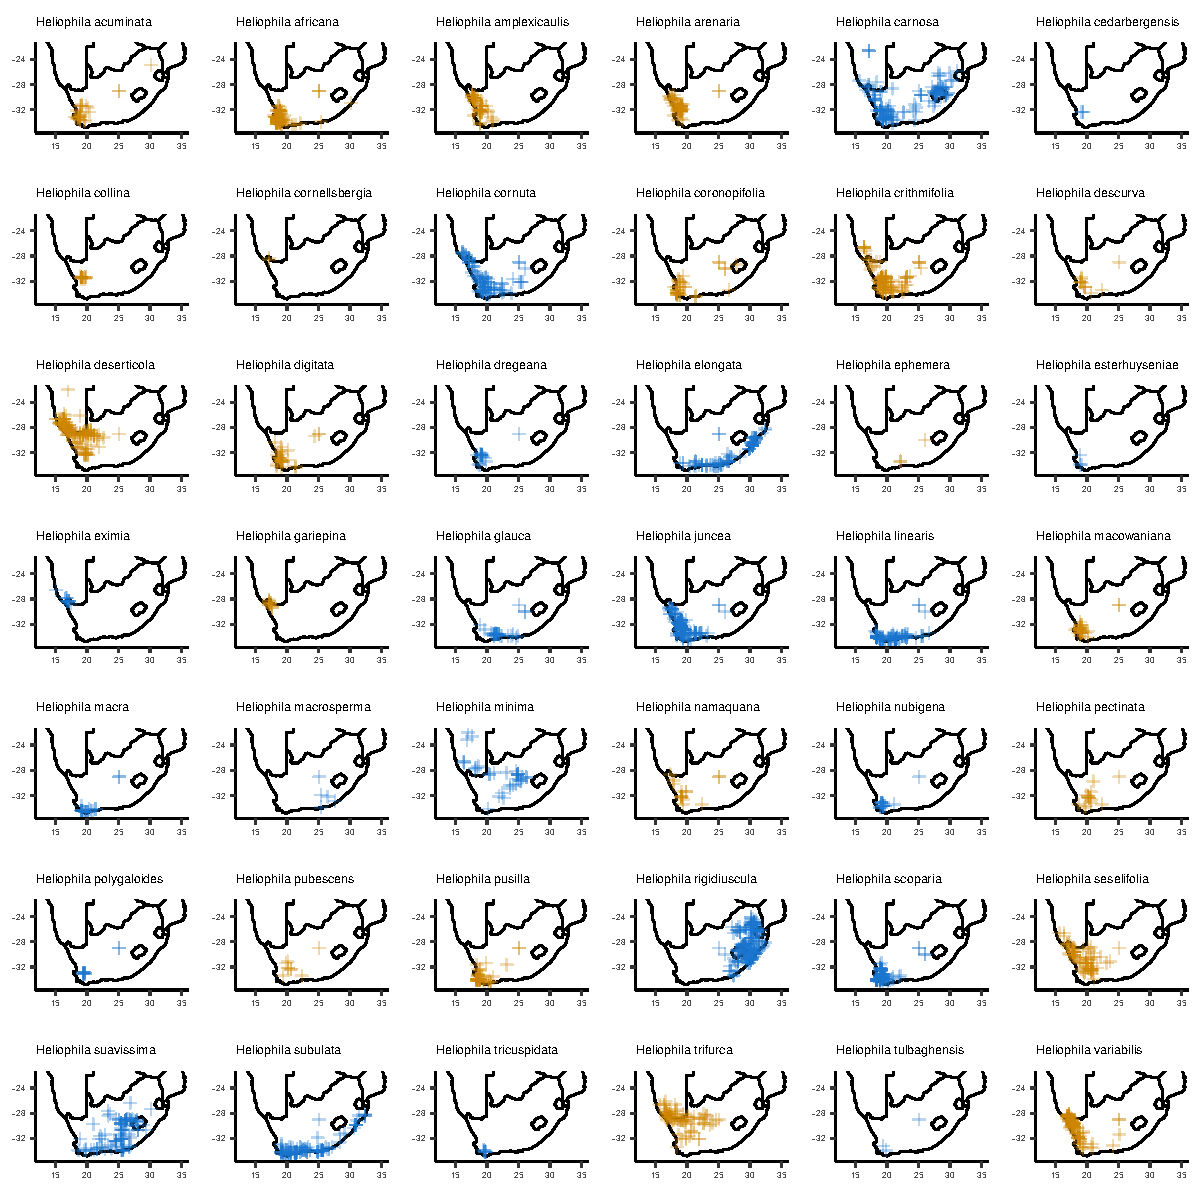
\includegraphics{../figures/speciesmaps.pdf}
\caption{\label{fig:speciesmaps}Maps of occurrence records for individual species.
Orange points indicate annual species. Blue points indicate perennial
species.}
\end{figure}


\end{document}
